\section{Performance}

This section describes the performance measurement of the system.
Firstly we present the metric used for measuring the performance in \autoref{sec:perf:fps}, then the bias involved when using this metric is discussed in \autoref{sec:perf:bias}.
\autoref{sec:perf:res} presents the results obtained and lastly \autoref{sec:perf:disc} discusses the results.

The performance was measured by implemententing the game application described in \autoref{circle-game} in both {\C} and {\rust} and recording a performance metric.
The performance metric chosen for the evaluation is the Frames Per Second, FPS.
This metric measures the amount of work/second.
The metric is simple and commonly used when measuring relative performance of realtime graphic applications.

\subsection{Performance Metric - Frames Per Second}
\label{sec:perf:fps}
To see what the FPS metric measures and how it affects the system measured we give a simple analysis of the execution pattern of the application in this section.

\begin{listing}[H]
  \begin{minted}{rust}
fn main() {
  init(); /* Run Microcontroller initialization */

  reset(); /* Reset the Game Environment */

  /* Game Loop */
  loop {
    let input = get_user_input(); // Get input from user buttons
    player.move(input);           // Move Player according to input
    obstical.move();              // Move obstical

    // check if collision occured
    if check_collision(player, obstical) {
      game_over(); // Report game is over to player
      reset();     // Reset the Game Environment
    }

    redraw_screen(); // Update contents on the LCD
  }
}
  \end{minted}
  \caption{}
  \label{lst:perf:game}
\end{listing}

The game consists of three phases; initialization, reset and the Game Loop.
As \autoref{lst:perf:game} suggests most of the work is done in the Game Loop.
The goal of the FPS metric is to measure how many iterations per second the program is able to perform.
\autoref{lst:perf:fps} shows the code added to measure the FPS metric.

\begin{listing}[H]
  \begin{minted}{rust}

static mut FRAME_COUNT = 0;
static mut LAST_FRAME_COUNT = 0;

fn main() {

  // ...
  setup_systick(); // Setup systick each second

  /* Game Loop */
  loop {

    // ...
    FRAME_COUNT += 1;
    draw_fps_to_screen(LAST_FRAME_COUNT);
  }
}

/* Interrupt handled once each second */
extern fn SysTick_Handler() {

  LAST_FRAME_COUNT = FRAME_COUNT;
  FRAME_COUNT = 0;
}
  \end{minted}
  \caption{}
  \label{lst:perf:fps}
\end{listing}

As can be seen in \autoref{lst:perf:fps} a frame counter is incremented each iteration of the Game Loop in the variable \code{FRAME\_COUNT}.
Each second this counter is stored in the \code{LAST\_FRAME\_COUNT} variable and reset to zero.
This ensures that each second the number of frames draw the last second is always held by the \code{LAST\_FRAME\_COUNT} variable.
This variable is printed on the screen on each iteration.

\subsection{Measurment Bias}
\label{sec:perf:bias}

When measuring performance one have to consider a number of biases that can and will occure while performing the measurement.
A Bias is an arbitrary external noise that might distort the result of the measurements.
Some of these biases can and should be elliminated before measuring, while others are harder or impossible to remove.
In a bare metal embedded system however, the biases are fewer compared to when running on an Operating System.
This is due to the fact that without an OS, the user application is the only "process" running on the CPU.

\autoref{itm:perf:bias} lists the biases after analysis of the game application.
\begin{figure}[H]
	\begin{itemize}
	\item User Input
	\item Random Number Generator
	\item Code for recording the performance metric
	\item Optimization Characteristics
	\end{itemize}
	\caption{Performance Bias for Game Application}
	\label{itm:perf:bias}
\end{figure}

Each bias from \autoref{itm:perf:bias} is discussed in the following paragraphs.

\paragraph{User Input} The game application was developed as a human playable game.
When measuring performance a desterministic result providing the same result when executing an identical program multiple times is preferable.
Getting the human player to make identical descisions at the same exact moment required by a game with contionous progress is a hard task.
In addition measurments are easier to perform when automated.
Therefore this bias was deemed to be big enough to eliminate completely.
This was done by implementing a simple artificial intellegence which emulates the user input.

\paragraph{Random Number Generator}
A Random Number Generator, RNG is used to generate a stream of seemingly random numbers.
The RNG is used to generate position for the obstacles the user has to avoid described in \autoref{sec:back:game}.
The rational for the User Input bias related to deterministic execution can be reiterated for a Random Number Generator, RNG.
As {\rust} implements its own RNG which does not depend on the C RNG, a bias can be observed between the platform.
This lead to the implementation of a simple deterministic RNG based the RNG for Doom.
This RNG contains a list of 256 seemingly random numbers.
Each time a number is requested by the application the RNG returns a number from the list and increments a internal index into the list.
When 256 numbers has been requested the index wraps around and returns the first number again.

\paragraph{Code for the measurement}
Often when measuring the performance of an application at a course granularity the measurement it self is a bias.
This is largely the case when measuring FPS as this adds profiling code to the actual application.
An alternative to FPS is be to measure the wall clock time or number of cpu cycles for an entire execution of a program.
In an game like the one considered here this could done by defining the game to end after a given number of levels and ensuring that all execution reaches this goal.
These kind of measurements are more relevant when the actual performance of the application is important.
Such applications can be the interrupt handler of a time critical stream of interrupt.
In these applications the success criteria is if the operation can be performed within the given deadline.
In this experiment we are interested in the releative performance between C code and {\rust} code.
Therefore the added bias by the FPS measurment is accetable as long as it is the same for both code bases.
In fact in this case we can reformulate the problem description of the Game to report the fps to user.
This is due to the fact that the process of measuring the FPS is similar in nature to the problem we are trying to measure.

\paragraph{Optimization Characteristics}
Various application performs different when subject to differnet optimizations.
This fact leads to a tradeoff when desciding the level of optimization to apply to the program.
To account for this bias we look at the performance metric for all optimization levels and do a analysis based on the best metric.
The bias here comes from the fact that we have chosen the FPS metric, which optimizes the game operation in the Game Loop.
Let us as an example say that the O2 would provide a FPS of 500 and O3 a FPS of 480.
This would suggest that the O2 was most suitable for this application, but if we analyse the execution speed of the initialzation and reset phase we might draw a different conclusion.
\todo{Should we account for this?}

\subsection{Results}
\label{sec:perf:res}

In this section the result obtained when measuring performance is presented.

\begin{figure}[H]
  \begin{center}
    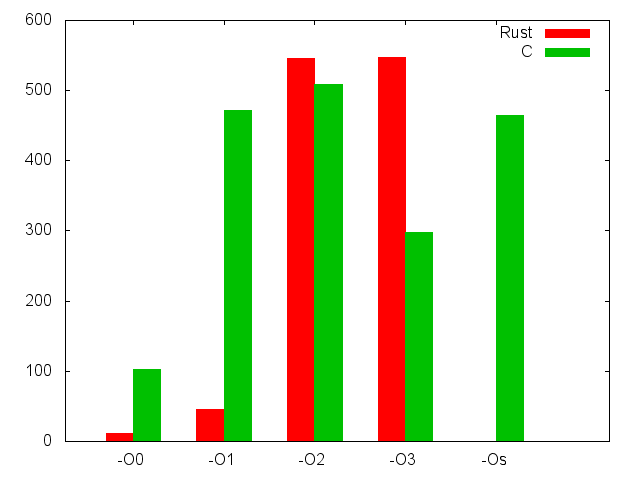
\includegraphics[scale=0.5]{results/plots/perf/perf.png}
  \end{center}
  \caption{Frame/Second achived by C and {\rust} code.}
  \label{fig:perf:res}
\end{figure}

\autoref{fig:perf:res} graphs the results for the performance measurements.
The Y axis shows the number of Frames Per Seconds achived by running the game on the optimization level given by the X axis.
We see that the C code is \~10x faster on O0 and O1, but {\rust} equates by providing a 1.07x speedup over C at O2.
C achives best performance at level O2 while {\rust} is slighly faster on O3 compared to O2.
The optimization Os for size is not available for {\rust} and is included for the discussion of size vs performance in \autoref{sec:res:size-v-perf}.
\todo{I'm thinking there will be a larger discussion taking all the results in consideration in the end of this chapter}

\subsection{Discussion}
\label{sec:perf:disc}
As \autoref{sec:perf:res} shows the performance of the application written in {\rust} not only matches the FPS performance of the C version, it also provides a speedup of 1.07x.
We also see that the optimiziations are more predictable on this application in relation to optimization level, with perf(Ox) > perf(Oy) when x > y.
This relationship does not hold for the C application where the perf(O1) > perf(O3).
The results for the C application shows that optimizing for size provides a higher performance enhancement than applying the most aggressive optimization.
